% Also note that the "draftcls" or "draftclsnofoot", not "draft", option
% should be used if it is desired that the figures are to be displayed in
% draft mode.
%
\documentclass[conference]{IEEEtran}
%
\ifCLASSINFOpdf
\usepackage[pdftex]{graphicx}
  % \DeclareGraphicsExtensions{.pdf,.jpeg,.png}
\else
  % \DeclareGraphicsExtensions{.eps}
\fi

% *** MATH PACKAGES ***
%
\usepackage[cmex10]{amsmath}

%\usepackage[caption=false]{caption}
\usepackage[font=footnotesize,caption=false]{subfig}

% --------------- USEPACKAGE agregados por guanucoluis ----------------

\usepackage[utf8]{inputenc}
\usepackage{multirow}
%\usepackage[english]{babel}
\usepackage{amssymb}
%\usepackage[pdftex]{graphicx}
\usepackage[hyphenbreaks]{breakurl}
\usepackage[hyphens]{url}

% ------------------------- Agregados por maxi ------------------------

\renewcommand{\abstractname}{Resumen}
\renewcommand{\figurename}{Figura}
\renewcommand{\tablename}{Tabla}
\renewcommand{\refname}{Referencias}
\hyphenation{de-sa-rro-llar de-sa-rro-llos de-sa-rro-llo clas-si-fi-can ne-ce-sa-ria-men-te dis-po-si-ti-vos in-te-gra-das es-pa-cio pre-sen-tan di-men-sio-nes di-fe-ren-tes in-dus-tri-al prin-ci-pa-les per-mi-ten com-pu-ta-do-ras pro-por-cio-na dis-po-si-ti-vo im-ple-men-tar par-ti-ci-pa-do di-gi-ta-les rui-do-sa he-rra-mien-tas}

% correct bad hyphenation here
\hyphenation{op-tical net-works semi-conduc-tor}


\begin{document}
%
% paper title
% can use linebreaks \\ within to get better formatting as desired
\title{Revisión -- Bubble Sort: An Archaeological Algorithmic Analysis}


% author names and affiliations
% use a multiple column layout for up to three different
% affiliations
\author{\IEEEauthorblockN{Luis Alberto Guanuco}
\IEEEauthorblockA{Algortímos y Patrones de Software\\
Especialidad en Sistemas Embebidos\\
Instituto Universitario Aeronáutico}
}

% make the title area
\maketitle


\begin{abstract}
El presente documento realiza una revisión de la publicación
\emph{Bubble Sort: An Archaeological Algorithmic Analysis}\cite{Astrachan}. Se
rescatan los puntos más importantes de las investigaciones realizadas
por \emph{Owen Astrachan}. El eje central de la publicación es la
revisión histórica del ordenamiento burbuja (\emph{bubble
  sort}). Se buscan los orígenes del algoritmos y la injustificable
vigencia del mismo en los ámbitos académicos informáticos.
\end{abstract}

\IEEEpeerreviewmaketitle

\section{Introducción}
\label{sec:intro}

El autor lleva adelante una investigación profunda de los orígenes del
algoritmo \emph{Bubble Sort}. Se plantea la situación de que el
algoritmo de ordenamiento más recurrente en las bibliografías clásicas
es el ordenamiento burbuja. Aunque se tengan fundamentos para excluir
a este algoritmo de los textos académicos.

\section{Los orígenes del algoritmo}
\label{sec:origen-alg}

El primer registro del algoritmo se da en el año 1956. En aquella
oportunidad no se lo presenta como \emph{Bubble Sort}, se la expone
como \emph{sorting by exchange}. Las publicaciones que le siguieron a
esta primera aparición del algoritmo siguieron con refiriéndose como
sorting by exchange. 
Una primera aparición del nombre \emph{Bubble Sort} se da en el año
1962.  Kenneth Iverson es el matemático que lo denomina con este
nombre al algoritmo de ordenamiento burbuja.
En el año 1963 el algoritmo ingreso en los repositorios de la ACM
(Association for Computing Machinery) donde el nombre designado fue
\emph{Shuttle Sort}. Luego de su publicación se encontraron
definiciones anexas al algoritmo como \emph{not free from
  errors}. Esto es consecuencia de los errores encontrados en las
implementaciones sucesivas. 

\subsection{Código del Bubble Sort}
\label{sec:origen-bubble-sort}

El autor del paper toma como referencia el código presentado en el
libro \emph{The Art of Computer Programming: Sorting and
  Searching}. El programa recorre todo el vector realizando
comparaciones de dos elementos sucesivos.
\begin{verbatim}
void BubbleSort(Vector a, int n)
{
  for(int j=n-1; j > 0; j--)
    for(int k=0; k < j; k++)
      if (a[k+1] < a[k])
        Swap(a,k,k+1);
}
\end{verbatim}

Sobre este código se presentan dos optimizaciones, vistas también en
la exposición de clases:
\begin{itemize}
\item Caso de tener un vector ordenado.
\item Alternar la  dirección del intercambio.
\end{itemize}

\subsection{Otros nombres para el Bubble Sort}
\label{sec:origen-otro-nombre}

Varias publicaciones posteriores a 1962 presentaron algoritmos con la
estructura del Bubble Sort. Entre ellos están el \emph{Push-Down
  Sort}, \emph{Jump-Down}, \emph{Selection Sort}, por nombrar
algunos. En la evolución de los algoritmos se dan a conocer trabajos
que comparan el Bubble Sort con otros algoritmos de ordenamiento.

\subsection{Los orígenes de popularidad}
\label{sec:origen-popu}

En el año 1971 se publican los resultados de una encuesta realizada
por el ACM sobre los algoritmos de ordenamiento existentes. Sobre el
Bubble Sort se concluyó,
\begin{quote}
El Bubble Sort es fácil de recordar y programar. Además requiere poco
tiempo para completar un simple recorrido.   
\end{quote}

Se relevaron más bibliografías y se encontraron trabajos que denotan
las limitantes del Bubble Sort. Estos se fundamentan en el orden de
complejidad del algoritmo ($O(n^2)$). El punto anterior hacer
referencia al consumo de recursos y el tiempo de respuesta del
algoritmo. Desde una perspectiva matemática Demuth demostró a través
de una tesis lo interesante del ordenamiento burbuja pero deja claro
que la implementación del algoritmo resulta insatisfactoria. 

\subsection{Mediciones de popularidad}
\label{sec:orig-med-pop}

Hasta el momento se dejó claro que el algoritmo del Bubble Sort tiene
un pobre performance pero se proporcionan evidencias de la vigencia
del algoritmo en bibliografías usadas en la actualidad. La Tabla
\ref{tab:pop} representa una evidencia de la popularidad del algoritmo
Bubble Sort. El proceso consistió en relevar los resultados de
búsquedas de diferentes algoritmos. Las muestras se tomaron en el años
2000 y 2002. 
\begin{table}[ht]
\renewcommand{\arraystretch}{1.3}
\caption{Popularidad de los algoritmos (basados en internet).}
\label{tab:pop}
\centering
\begin{tabular}{|c|r|r|}
\hline
\textbf{algoritmo} & \textbf{\# búsq. 2000} & \textbf{\# búsq. 2002} \\
\hline
Quick     & 26,780 & 80,200 \\
Merge     & 13,330 & 33,500 \\
Heap      & 9,830  & 22,960 \\
Bubble    & 12,400 & 33,800 \\
Insertion & 8,450  & 21,870 \\
Selection & 6,720  & 20,600 \\
Shell     & 4,540  & 8,620  \\
\hline
\end{tabular}
\end{table}

Analizando las estadísticas proporcionadas, Bubble Sort no el
algoritmo con mayor recurrencia. Esto resulta satisfactorio pues
existen muchos otros algoritmos con mayor eficiencia. Aún así se
encuentra en el segundo o tercer lugar entre los más recurridos. 

\section{Características de funcionamiento}
\label{sec:car-func}

Continuando con la misma línea, el autor del trabajo realiza estudios
comparativos del algoritmo Bubble Sort con otros posteriores. En esta
sección parte de la publicación considera los aspectos de la
implementación tanto en la complejidad del código como el tiempo de
ejecución. Estos parámetros son fueron analizados en un artículo
publicado por Helstead en 1977. Estas métricas se basan en las cuentas
sobre los operaciones sobre el código. La Tabla \ref{tab:measure}
representa la relación entre \emph{Dificultad} y \emph{Esfuerzo} para
varios algoritmos de ordenamiento. La \emph{dificultad} se refiere a
qué tan duro es realizar la implementación. Mientras que el
\emph{esfuerzo} se refiere al trabajo necesario para convertir el
algoritmo en un programa.
\begin{table}[ht]
  \renewcommand{\arraystretch}{1.3}
  \caption{Complejidades pedidas por Halstead de ordenamientos.}
  \label{tab:measure}
  \centering
  \begin{tabular}{|c|r|r|}
    \hline
    \textbf{algoritmo} & \textbf{Dif.} & \textbf{Esf.} \\
    \hline
    Bubble    & 17.25 & 4165 \\
    Jump-down & 14.38 & 3828 \\
    Select    & 15.95 & 4242 \\
    Insert    & 23.20 & 6652 \\
    Quick     & 7.88  & 3157 \\
    Partition & 12.07 & 1522 \\
    \hline
  \end{tabular}
\end{table}

El autor de la publicación revisada expone referencias concretas sobre
el bajo performance del algoritmo Bubble Sort. En la Figura
\ref{fig:performance} se presentan los tiempos que demandan diferentes
algoritmos de ordenamiento en función de la cantidad de elementos de
entrada. 
\begin{figure}[ht]
  \centering
  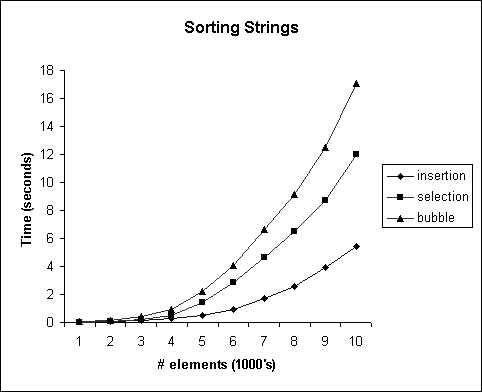
\includegraphics[width=0.45\textwidth]{img/performance}
  \caption{Ordenamiento de strings.}
  \label{fig:performance}
\end{figure}

\section{Conclusiones del Autor}
\label{sec:conc}
Más allá de los análisis realizados el mejor algoritmo de ordenamiento
a implementar siempre será el proporcionado por las librerías del
lenguaje a utilizar (Java, C++, etc.). En análisis de los algoritmos
de ordenamiento, aun que parezcan sencillos, muestra los diferentes
resultados para situaciones distintas. En los primeros años de la
enseñanza de programación es recurrente el uso del Bubble Sort. Sí
bien se justifica su uso por la aparente \emph{sencillez}, aquí se
emite una fuerte crítica a elegir otro tipo de algoritmo que sea lo
suficientemente sencillo y complejo. El trabajo escrito por \emph{Owen
Astrachan} confirma el bajo performance en lo que refiere a la
codificación y consumo de recursos en su ejecución.

\begin{thebibliography}{1}
\bibitem{Astrachan}
  Owen~Astrachan, \emph{Bubble Sort: An Archaeological Algorithmic
    Analysis}. Computer Science Departament, Duke University. 
\end{thebibliography}

% that's all folks
\end{document}


